\section{联合分布}
\label{sec:rvc-joint}

两台传感器各自的读数规律，第~\ref{chap:random-variables}章已经会写：每台都有一张概率表。要回答“两台同时报偏高”这样的问题，需要的却是读数\emph{对}的概率。这一节先说明几个随机变量怎样放进同一次试验，再用概率表、密度和分布函数记录它们的共同规律，最后从共同规律中取出单个分量的规律。

\paragraph{同一次试验中的几个随机变量}
随机变量是样本空间$\Omega$上的函数：试验给出一个样本点$\omega$，随机变量把它变成一个数。几个随机变量要能“一起取值”，必须定义在同一个$\Omega$上，这样同一个$\omega$同时决定它们全部的值。

掷两颗均匀骰子是最直接的例子。样本空间由$36$个等可能的有序对$(i,j)$组成，$i$是第一颗的点数，$j$是第二颗的点数。令$X$为第一颗的点数，$M$为两颗中较大的点数，即
\[
 X(i,j)=i,\qquad M(i,j)=\max\{i,j\}.
\]
每个样本点同时给出一对值$(X,M)$。事件$\{X=4,\,M=4\}$由第一颗为$4$、第二颗不超过$4$的四个样本点组成，概率是$4/36$；事件$\{X=2,\,M=5\}$只含样本点$(2,5)$，概率是$1/36$。

把$36$个样本点按它们给出的$(X,M)$分组，每组的点数除以$36$，就得到每一对取值的概率，见图~\ref{fig:rvc-dice-map}。表中右下方的空格表示$M<X$的取值对，它们不可能出现，因为较大点数不会小于第一颗的点数。这张表记录的正是“两个量怎样一起取值”。

\begin{BookInlineFigure}
  \centering
  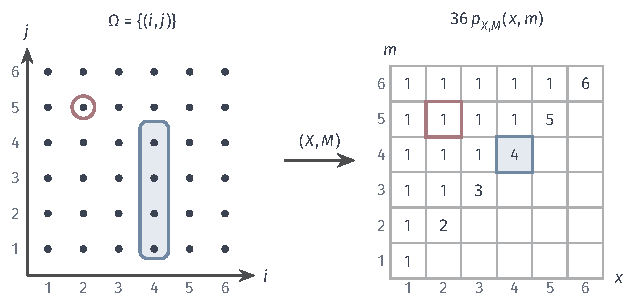
\includegraphics[width=107mm]{figures/07-probability/01-elementary-probability/tikz/rvc-dice-map/figure.pdf}
  \caption{从样本点到联合概率表。左侧是两颗骰子的$36$个样本点，横坐标为第一颗点数$i$，纵坐标为第二颗点数$j$。右侧格子$(x,m)$中的数是满足$X=x$、$M=m$的样本点个数，除以$36$即为概率。蓝框中的四个样本点都给出$(X,M)=(4,4)$，红圈中的样本点$(2,5)$单独给出$(2,5)$；空格的概率为零。}
  \label{fig:rvc-dice-map}
\end{BookInlineFigure}

\begin{definition}[随机向量与联合分布]
\label{def:rvc-random-vector}
设$X_1,\dots,X_d$是定义在同一样本空间$\Omega$上的随机变量。把它们排成列向量
\begin{equation}
 \bm{X}=(X_1,\dots,X_d)^{\top},
 \label{eq:rvc-random-vector}
\end{equation}
称为$d$维\term{随机向量}（random vector）。对$\mathbb{R}^{d}$中的集合$A$，事件$\{\bm{X}\in A\}$由使$\bm{X}(\omega)\in A$的样本点组成；这些事件的概率$\mathbb{P}(\bm{X}\in A)$合起来称为$\bm{X}$的\term{联合分布}（joint distribution）。
\end{definition}

本部分只处理能用求和或普通积分算出概率的集合$A$，例如有限点集、矩形和卷二能够积分的平面区域；对哪些集合赋予概率的一般规定在第~\ref{chap:probability-spaces}章给出。随机向量与它的联合分布是两件事，这一点和一元情形相同。$\bm{X}$是$\Omega$上的函数，回答“这次试验得到哪个向量”；联合分布只回答“各个区域的向量出现的概率是多少”。两颗骰子的$(X,M)$和后面许多问题只需要联合分布，但只有回到$\Omega$，才能说清几个量为什么会一起变化。

\paragraph{联合概率表}
两个变量都只取有限个或可数个值时，每一对取值的概率就足以计算一切。仍用大写字母表示随机变量、小写字母表示取值，定义
\begin{equation}
 p_{X,Y}(x,y)=\mathbb{P}(X=x,\,Y=y),
 \label{eq:rvc-joint-pmf}
\end{equation}
称为$(X,Y)$的\term{联合质量函数}（joint probability mass function）。它非负，对全部取值对求和等于$1$。

事件$\{(X,Y)\in A\}$可以按取值对拆成互斥的单点事件，由可加性，
\begin{equation}
 \mathbb{P}\bigl((X,Y)\in A\bigr)=\sum_{(x,y)\in A}p_{X,Y}(x,y).
 \label{eq:rvc-joint-pmf-event}
\end{equation}
把概率想象成总量为$1$的质量，联合质量函数就是把这份质量分配到平面上的一些格点；任何联合事件的概率，等于事件圈住的格点上的质量之和。

回到两台传感器。设第一台的档位为$X$，第二台为$Y$，作为教学示例，取图~\ref{fig:rvc-sensor-table}中的概率表。九个数之和为$1$。两台不会一台读$0$、另一台读$2$，相邻档位的组合各占$0.10$，对角线上的组合各占$0.20$：两台读数倾向于一致，但并不总是一致。

\begin{BookInlineFigure}
  \centering
  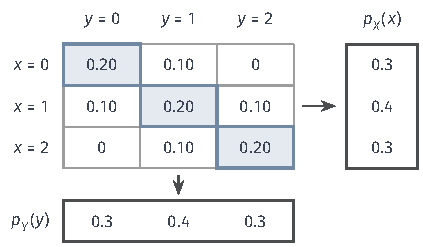
\includegraphics[width=72mm]{figures/07-probability/01-elementary-probability/tikz/rvc-sensor-table/figure.pdf}
  \caption{两台传感器档位的联合概率表。行对应第一台的档位$x$，列对应第二台的档位$y$。浅蓝格子组成事件$\{X=Y\}$；右侧方框是各行之和$p_X(x)$，下方方框是各列之和$p_Y(y)$。}
  \label{fig:rvc-sensor-table}
\end{BookInlineFigure}

由式~\eqref{eq:rvc-joint-pmf-event}，读数一致的概率是对角线三格之和，读数之和至少为$3$的概率是右下角三格之和：
\[
 \mathbb{P}(X=Y)=0.20+0.20+0.20=0.60,
\]
\[
 \mathbb{P}(X+Y\geq 3)=p_{X,Y}(1,2)+p_{X,Y}(2,1)+p_{X,Y}(2,2)=0.40.
\]
两台同时报偏高的概率就是一个格子：$\mathbb{P}(X=2,\,Y=2)=0.20$。这些问题都无法只用每台各自的概率表回答。

\paragraph{联合密度}
如果两个量连续取值，单个点的概率为零，概率表不再适用。一元情形用密度表示单位长度上的质量；平面上相应地用单位面积上的质量。

\begin{definition}[联合密度]
\label{def:rvc-joint-density}
设$f_{X,Y}$是平面上的非负函数。若对每个矩形$R=[a_1,b_1]\times[a_2,b_2]$都有
\begin{equation}
 \mathbb{P}\bigl((X,Y)\in R\bigr)=\iint_{R}f_{X,Y}(x,y)\,\mathrm{d}x\,\mathrm{d}y,
 \label{eq:rvc-joint-density}
\end{equation}
则称$f_{X,Y}$为$(X,Y)$的\term{联合密度}（joint density）。
\end{definition}

矩形概率确定以后，整个联合分布也就确定了：对卷二能够积分的区域$A$，$\mathbb{P}((X,Y)\in A)$同样等于$f_{X,Y}$在$A$上的积分。这一事实的证明需要第~\ref{chap:probability-spaces}章的工具，这里直接使用。多重积分、累次积分以及无界区域上非负函数积分的计算规则，可参考\BookChapterRef{chap:region-integrals}{卷二第24章“区域积分”}。取$A$为整个平面，可知联合密度的积分等于$1$。

联合密度本身不是概率。在点$(x,y)$附近取边长为$h$和$k$的小矩形，若$f_{X,Y}$在该点附近连续，矩形的概率约为$f_{X,Y}(x,y)\,hk$；密度大的地方，同样面积上的概率多。$d$维情形把二重积分换成$d$重积分，把面积换成体积即可。

现在建立贯穿全章的连续例子。令点$(X,Y)$在三角形$T=\{(x,y):0\leq y\leq x\leq 1\}$上均匀分布，即
\begin{equation}
 f_{X,Y}(x,y)=\begin{cases}2,&0\leq y\leq x\leq 1,\\0,&\text{其他}.\end{cases}
 \label{eq:rvc-triangle-density}
\end{equation}
三角形的面积是$1/2$，所以常数取$2$才能使总积分为$1$。“均匀”指同样面积的区域只要都落在三角形内，概率就相同。

求$\mathbb{P}(X+Y\leq 1)$。事件在三角形内对应的部分是顶点为$(0,0)$、$(1,0)$、$(1/2,1/2)$的小三角形，见图~\ref{fig:rvc-triangle-density}(a)。固定$y\in[0,1/2]$，$x$从$y$走到$1-y$，先对$x$积分：
\[
 \mathbb{P}(X+Y\leq 1)=\int_{0}^{1/2}\!\!\int_{y}^{1-y}2\,\mathrm{d}x\,\mathrm{d}y
 =\int_{0}^{1/2}2(1-2y)\,\mathrm{d}y.
\]
再对$y$积分，
\[
 \int_{0}^{1/2}2(1-2y)\,\mathrm{d}y=\Bigl[2y-2y^{2}\Bigr]_{0}^{1/2}=\frac12 .
\]
密度是常数时，概率就是“事件区域面积乘以$2$”：小三角形的面积是$1/4$，结果相同。

\begin{BookInlineFigure}
  \centering
  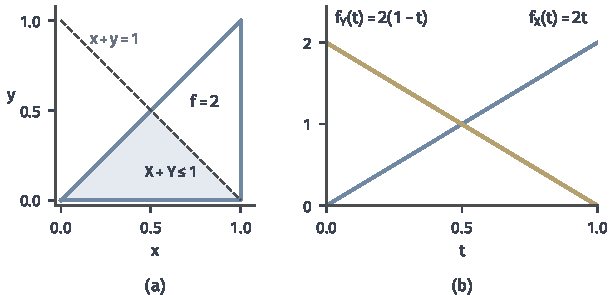
\includegraphics[width=104mm]{figures/07-probability/01-elementary-probability/matplotlib/rvc-triangle-density/figure.pdf}
  \caption{三角形上的均匀密度。(a)蓝线围成的三角形内密度为$2$，其外为$0$；浅蓝区域是事件$\{X+Y\leq 1\}$，概率$1/2$，虚线为$x+y=1$。(b)两个边缘密度：$f_X(t)=2t$（蓝）与$f_Y(t)=2(1-t)$（黄），$t\in[0,1]$。}
  \label{fig:rvc-triangle-density}
\end{BookInlineFigure}

\paragraph{联合分布函数}
概率表只适用于离散情形，联合密度只适用于连续情形。与一元情形一样，分布函数对两类模型都有意义。对$d$维随机向量定义\term{联合分布函数}（joint distribution function）
\begin{equation}
 F_{\bm{X}}(\bm{x})=\mathbb{P}(X_1\leq x_1,\dots,X_d\leq x_d),\qquad \bm{x}\in\mathbb{R}^{d}.
 \label{eq:rvc-joint-cdf}
\end{equation}
二维时，$F_{X,Y}(x,y)$是点$(x,y)$左下方整个象限的概率，见图~\ref{fig:rvc-cdf-rectangle}(a)。

矩形的概率可以由四个角上的分布函数值算出。设$a_1<b_1$，$a_2<b_2$，记$R=(a_1,b_1]\times(a_2,b_2]$。从象限$\{X\leq b_1,Y\leq b_2\}$中去掉$\{X\leq a_1,Y\leq b_2\}$和$\{X\leq b_1,Y\leq a_2\}$，两者的公共部分$\{X\leq a_1,Y\leq a_2\}$被去掉了两次，需要加回一次，于是
\begin{equation}
 \begin{aligned}
 \mathbb{P}\bigl((X,Y)\in R\bigr)
 &=F_{X,Y}(b_1,b_2)-F_{X,Y}(a_1,b_2)\\
 &\quad-F_{X,Y}(b_1,a_2)+F_{X,Y}(a_1,a_2).
 \end{aligned}
 \label{eq:rvc-rectangle}
\end{equation}
图~\ref{fig:rvc-cdf-rectangle}(b)中四个角上的符号就是这四项的正负号。由此可见，分布函数确定全部矩形的概率，从而确定联合分布。

\begin{BookInlineFigure}
  \centering
  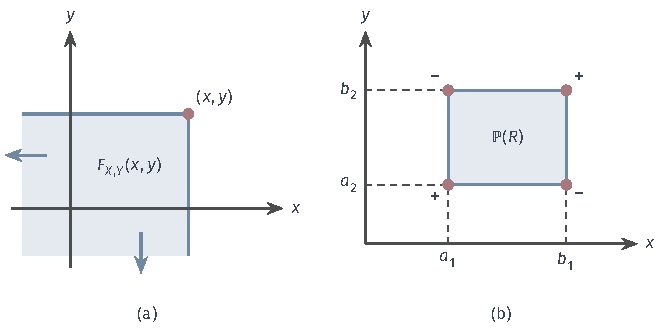
\includegraphics[width=112mm]{figures/07-probability/01-elementary-probability/tikz/rvc-cdf-rectangle/figure.pdf}
  \caption{联合分布函数与矩形概率。(a)$F_{X,Y}(x,y)$是红点左下方象限（浅蓝，向左、向下无界）的概率。(b)矩形$R=(a_1,b_1]\times(a_2,b_2]$的概率等于四个角上分布函数值的带符号和，符号标在各角旁。}
  \label{fig:rvc-cdf-rectangle}
\end{BookInlineFigure}

对三角形模型，$0\leq y\leq x\leq 1$时，左下方象限与三角形的交是梯形$\{(s,t):t\leq s\leq x,\ t\leq y\}$，面积为$xy-y^{2}/2$，乘以密度$2$得
\[
 F_{X,Y}(x,y)=2xy-y^{2},\qquad 0\leq y\leq x\leq 1 .
\]
$0\leq x<y\leq 1$时，象限与三角形的交是$\{t\leq s\leq x\}$，$F_{X,Y}(x,y)=x^{2}$。代入式~\eqref{eq:rvc-rectangle}检验矩形$(1/2,1]\times(0,1/2]$的概率：
\[
 F_{X,Y}(1,\tfrac12)-F_{X,Y}(\tfrac12,\tfrac12)-F_{X,Y}(1,0)+F_{X,Y}(\tfrac12,0)
 =\tfrac34-\tfrac14-0+0=\tfrac12 .
\]
这个正方形整个落在三角形内，面积$1/4$乘以密度$2$也是$1/2$。

\paragraph{边缘分布}
有了联合分布，常常又只关心其中一个分量，例如只问第一台传感器的读数。事件$\{X=x\}$可以按$Y$的取值拆成互斥事件$\{X=x,Y=y\}$的并，由可加性得到
\begin{equation}
 p_X(x)=\sum_{y}p_{X,Y}(x,y),\qquad p_Y(y)=\sum_{x}p_{X,Y}(x,y).
 \label{eq:rvc-marginal-pmf}
\end{equation}
在概率表上，这就是按行求和或按列求和。图~\ref{fig:rvc-sensor-table}中两台传感器的规律相同：
\[
 p_X=p_Y=(0.3,\,0.4,\,0.3).
\]

有联合密度时，取矩形$[a,b]\times[-c,c]$，令$c\to\infty$，先对$y$积分，得到
\[
 \mathbb{P}(a\leq X\leq b)=\int_{a}^{b}\Bigl(\int_{-\infty}^{\infty}f_{X,Y}(x,y)\,\mathrm{d}y\Bigr)\mathrm{d}x .
\]
这里交换顺序与取极限的依据是非负函数的累次积分。上式说明括号里的函数就是$X$的密度：
\begin{equation}
 f_X(x)=\int_{-\infty}^{\infty}f_{X,Y}(x,y)\,\mathrm{d}y,\qquad f_Y(y)=\int_{-\infty}^{\infty}f_{X,Y}(x,y)\,\mathrm{d}x.
 \label{eq:rvc-marginal-density}
\end{equation}
由联合分布得到的单个分量的分布称为\term{边缘分布}（marginal distribution），对其余分量求和或积分的操作称为\term{边缘化}（marginalization）。名称来自概率表：行和与列和写在表的边上。

对三角形模型，固定$x\in[0,1]$，密度只在$0\leq y\leq x$上取$2$；固定$y\in[0,1]$，密度只在$y\leq x\leq 1$上取$2$。于是
\[
 f_X(x)=\int_{0}^{x}2\,\mathrm{d}y=2x,\qquad f_Y(y)=\int_{y}^{1}2\,\mathrm{d}x=2(1-y),
\]
两式都在$[0,1]$上成立，见图~\ref{fig:rvc-triangle-density}(b)。$X$的质量偏向$1$，$Y$的质量偏向$0$：三角形在右侧竖得高，在下方铺得宽。

两颗骰子的例子也可以这样核对。图~\ref{fig:rvc-dice-map}右表中第$m$行有$m-1$个$1$和一个$m$，按行求和得到较大点数的边缘分布
\[
 p_M(m)=\frac{(m-1)+m}{36}=\frac{2m-1}{36},\qquad m=1,\dots,6 .
\]
六个值依次为$1/36,3/36,\dots,11/36$，和为$1$；较大点数偏向大的值。直接从样本空间看，$\{M\leq m\}$要求两颗都不超过$m$，概率为$m^{2}/36$，相邻两项相减同样得到$(2m-1)/36$。

$d$维时规则相同：保留哪些分量，就对其余全部分量求和或积分。例如三维密度$f(x_1,x_2,x_3)$对$x_3$积分得到$(X_1,X_2)$的二维边缘密度，再对$x_2$积分得到$X_1$的边缘密度。用分布函数表示，边缘分布函数是把其余坐标推向$+\infty$的极限，例如$F_X(x)=\lim_{y\to\infty}F_{X,Y}(x,y)$。

\paragraph{相同的边缘，不同的联合}
边缘化把其他分量的信息汇总掉了，这一步一般不能逆转。图~\ref{fig:rvc-same-marginals}把传感器表与另一张表并排放置：右表的每个格子取行和与列和的乘积。两张表的行和、列和完全一样，联合规律却不同。

\begin{BookInlineFigure}
  \centering
  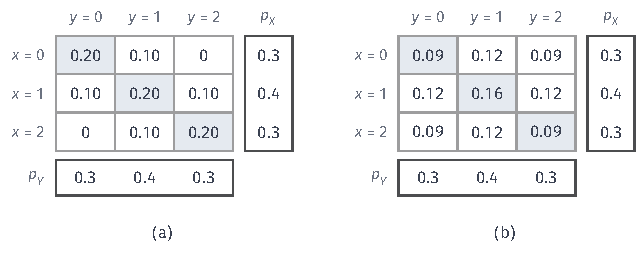
\includegraphics[width=108mm]{figures/07-probability/01-elementary-probability/tikz/rvc-same-marginals/figure.pdf}
  \caption{边缘相同、联合不同的两张概率表。(a)两台传感器的概率表。(b)每格取$p_X(x)p_Y(y)$得到的表。两表的行和与列和都是$(0.3,0.4,0.3)$；浅蓝格子组成事件$\{X=Y\}$，概率分别为$0.60$和$0.34$。}
  \label{fig:rvc-same-marginals}
\end{BookInlineFigure}

右表中读数一致的概率是
\[
 0.09+0.16+0.09=0.34,
\]
远小于左表的$0.60$；右表还允许一台读$0$、另一台读$2$，概率各为$0.09$。只看每台传感器各自的规律，分不出这两种情况。

连续情形也一样。对$\theta\in[-1,1]$，在单位正方形上令
\[
 f_{\theta}(x,y)=1+\theta(1-2x)(1-2y),\qquad 0\leq x,y\leq 1 .
\]
因为$\lvert(1-2x)(1-2y)\rvert\leq 1$，这个函数非负。对$y$积分时，$\int_{0}^{1}(1-2y)\,\mathrm{d}y=0$，所以
\[
 \int_{0}^{1}f_{\theta}(x,y)\,\mathrm{d}y=1+\theta(1-2x)\cdot 0=1 .
\]
同理对$x$积分也得$1$。于是每个$\theta$都给出一个联合密度，两个边缘都是$\operatorname{Unif}(0,1)$。图~\ref{fig:rvc-fgm}中，$\theta=1$时质量偏向两个分量同小或同大的角落，$\theta=-1$时偏向一小一大的角落。

\begin{BookInlineFigure}
  \centering
  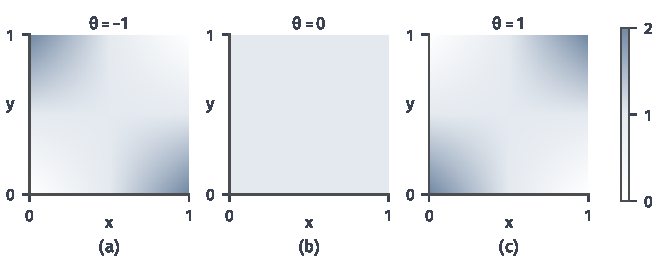
\includegraphics[width=112mm]{figures/07-probability/01-elementary-probability/matplotlib/rvc-fgm/figure.pdf}
  \caption{同样以$\operatorname{Unif}(0,1)$为两个边缘的三个联合密度$f_{\theta}(x,y)=1+\theta(1-2x)(1-2y)$。颜色由白到蓝表示密度由$0$到$2$。(a)$\theta=-1$。(b)$\theta=0$，密度处处为$1$。(c)$\theta=1$。}
  \label{fig:rvc-fgm}
\end{BookInlineFigure}

因此，单独知道每个分量的分布，不足以回答涉及几个分量共同取值的问题。联合分布在边缘之外还记录了分量之间的联系。下一节先研究联系“最弱”的情形：联合分布恰好可以由边缘拼出来。
